% !TEX TS-program = xelatex
% !TEX encoding = UTF-8
% !Mode:: "TeX:UTF-8"

\documentclass[onecolumn,twoside]{UWMadisonHomework}

\usepackage{blindtext}
\author{}
\clsID{NaN}
\title{ECE 845 Final Project}
\coursecode{ECE 845}
\coursename{Ensemble Monte Carlo Simulation}

\begin{document}
\maketitle

\definecolor{darkgreen}{rgb}{0.0, 0.39, 0.0} % RGB values for dark green
\definecolor{ForestGreen}{rgb}{0.13, 0.55, 0.13}

\section*{Problem 1}
To perform the simulation, I choose 100000 particles and the total flight time for each particle is around $30$ fs so that they can reach the steady state. The histogram of the initial energy and initial $k_z$ of the particles is shown below.
\begin{figure}[htbp]
  \centering
  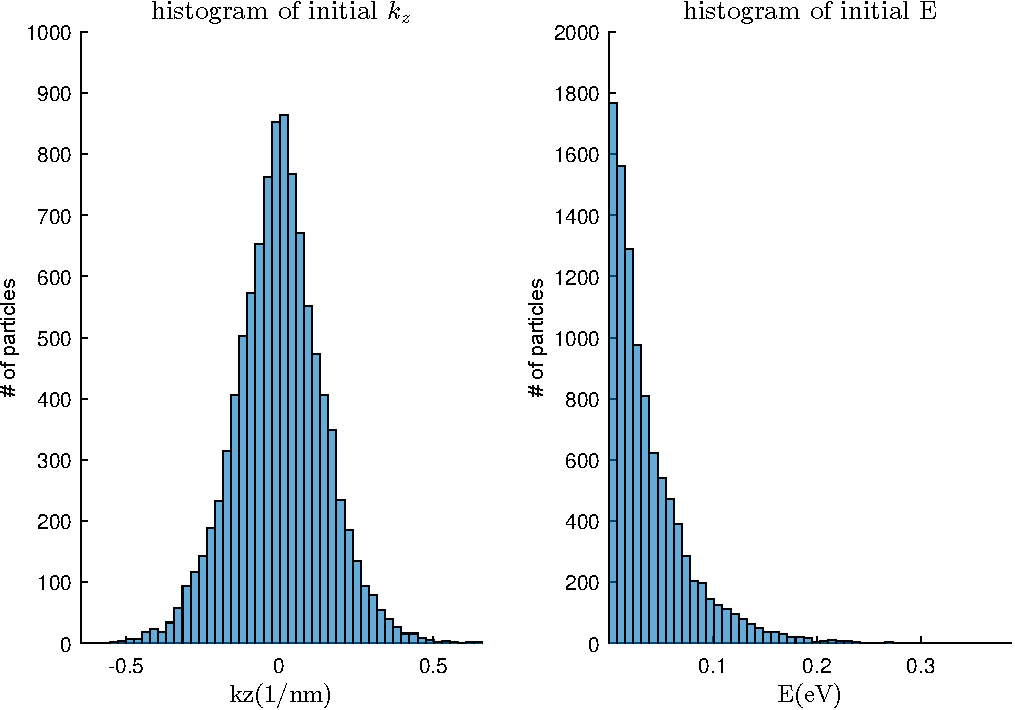
\includegraphics[width=0.75\textwidth]{figures/20250512_194456_histogram.pdf}
  \caption{}
\end{figure}

The scattering rates of different scattering mechanisms as a function of energy at three valleys, along with the accumulated scattering rates are given below.
\begin{figure}[htbp]
  \centering
  \begin{subfigure}[b]{0.45\textwidth}
      \centering
      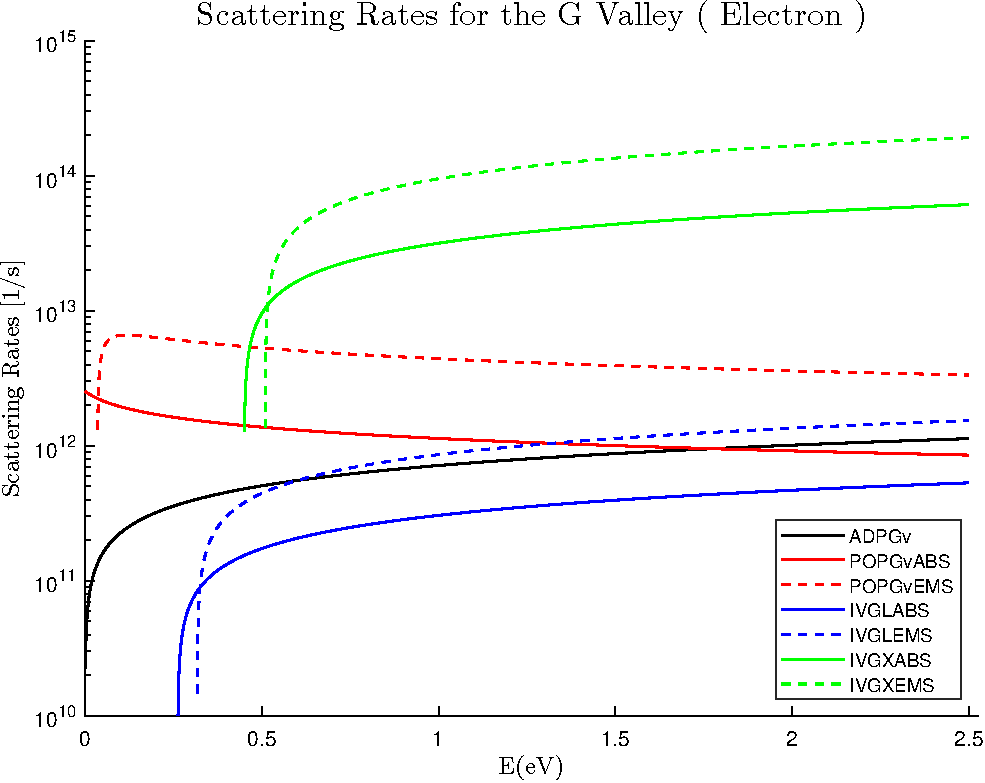
\includegraphics[width=\textwidth]{figures/20250512_130907_scattering_rate_G_valley.pdf}
      \caption{scattering rates for G valley}
      %\label{fig:graphene-band-surfaces2}
  \end{subfigure}
  \hfill % 增加水平间距
  \begin{subfigure}[b]{0.45\textwidth}
      \centering
      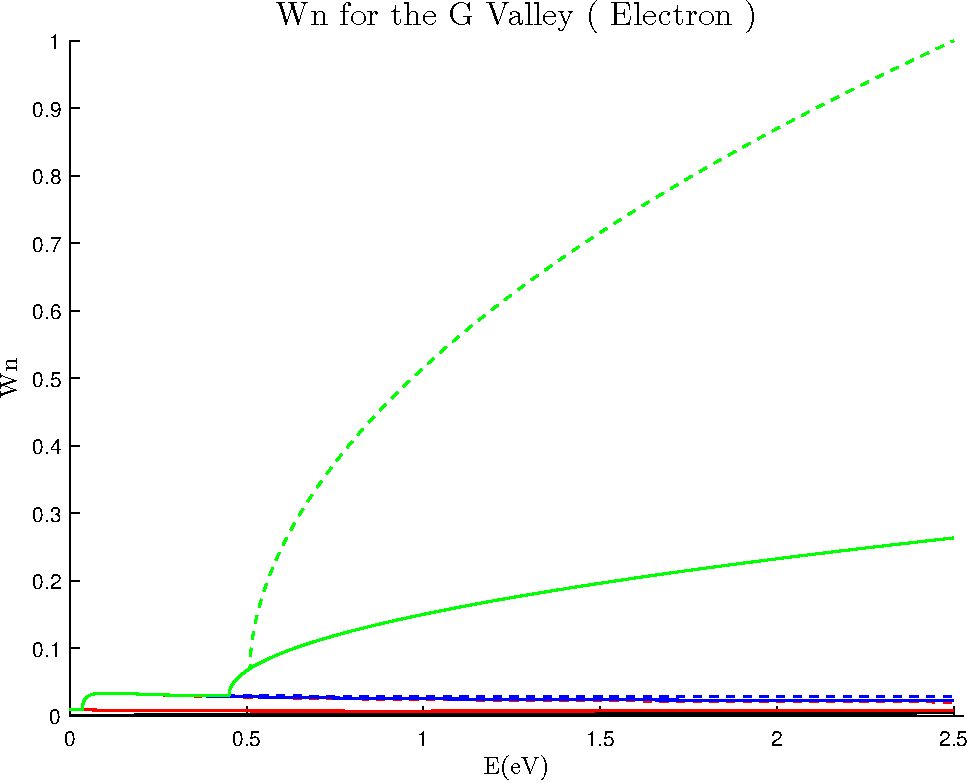
\includegraphics[width=\textwidth]{figures/20250512_130907_Wns_G_valley.pdf}
      \caption{accumulated scattering rates for G valley}
      %\label{fig:graphene-band-surfaces2}
  \end{subfigure}
\end{figure}

\begin{figure}[htbp]
  \centering
  \begin{subfigure}[b]{0.45\textwidth}
      \centering
      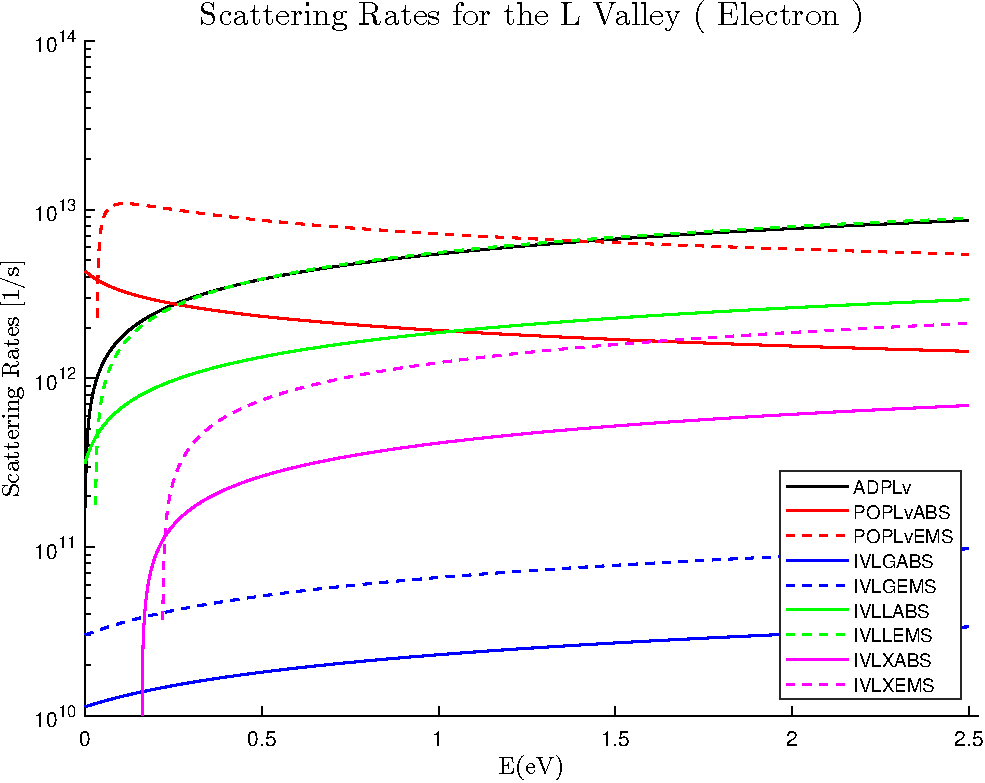
\includegraphics[width=\textwidth]{figures/20250512_130907_scattering_rate_L_valley.pdf}
      \caption{scattering rates for L valley}
      %\label{fig:graphene-band-surfaces2}
  \end{subfigure}
  \hfill % 增加水平间距
  \begin{subfigure}[b]{0.45\textwidth}
      \centering
      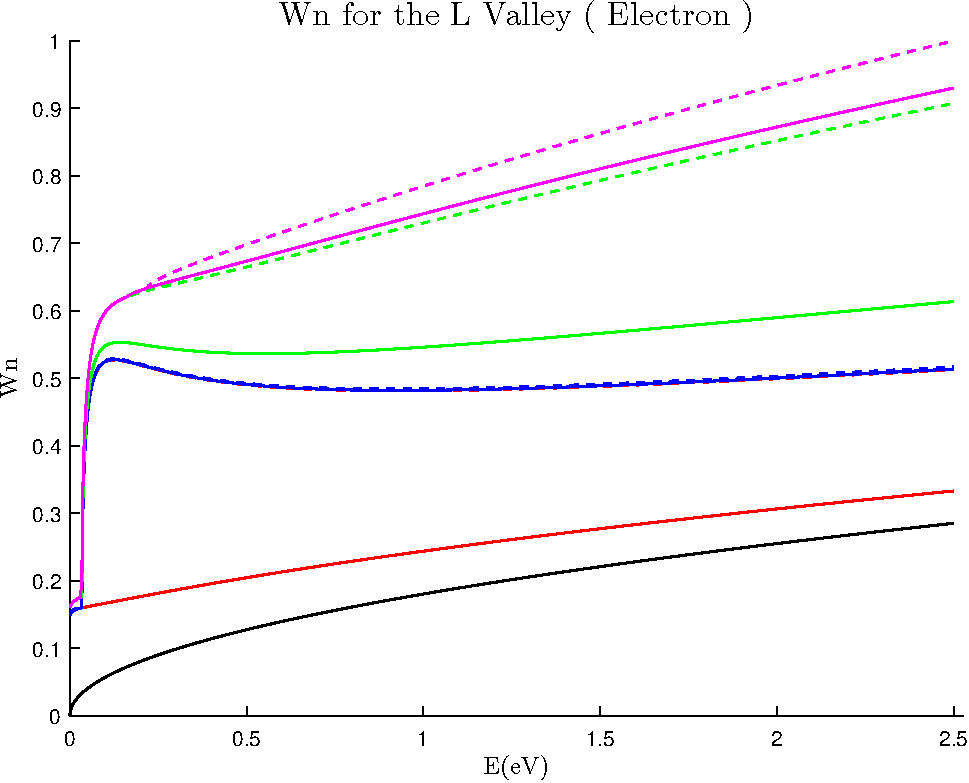
\includegraphics[width=\textwidth]{figures/20250512_130907_Wns_L_valley.pdf}
      \caption{accumulated scattering rates for L valley}
      %\label{fig:graphene-band-surfaces2}
  \end{subfigure}
\end{figure}

\begin{figure}[htbp]
  \centering
  \begin{subfigure}[b]{0.45\textwidth}
      \centering
      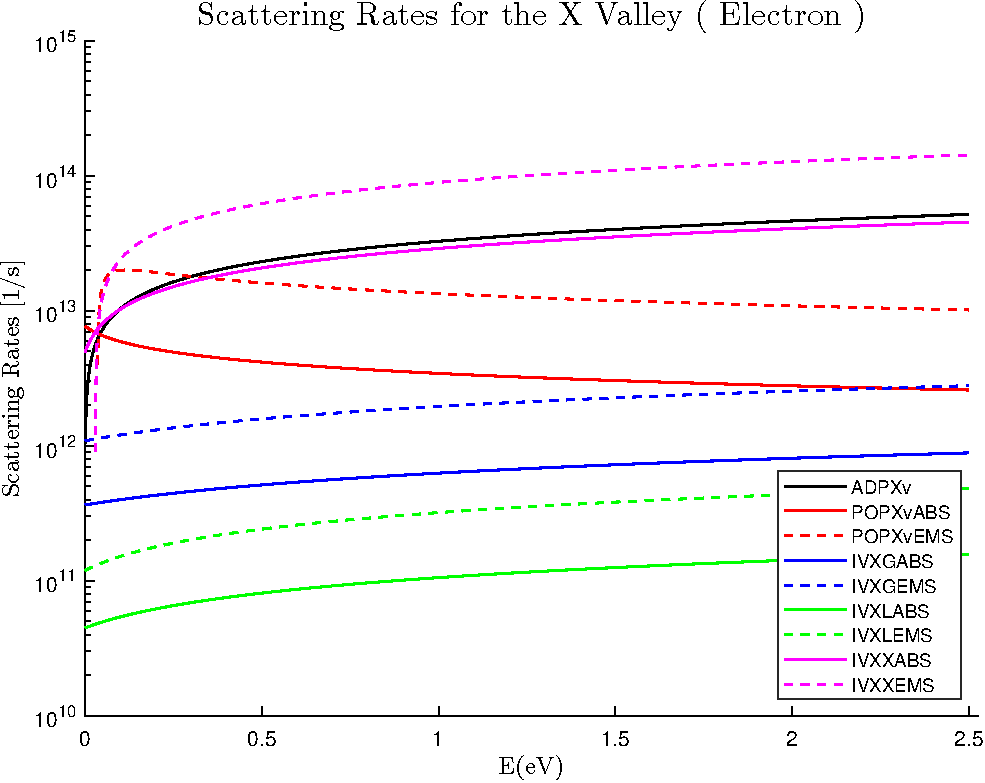
\includegraphics[width=\textwidth]{figures/20250512_130907_scattering_rate_X_valley.pdf}
      \caption{scattering rates for X valley}
      %\label{fig:graphene-band-surfaces2}
  \end{subfigure}
  \hfill % 增加水平间距
  \begin{subfigure}[b]{0.45\textwidth}
      \centering
      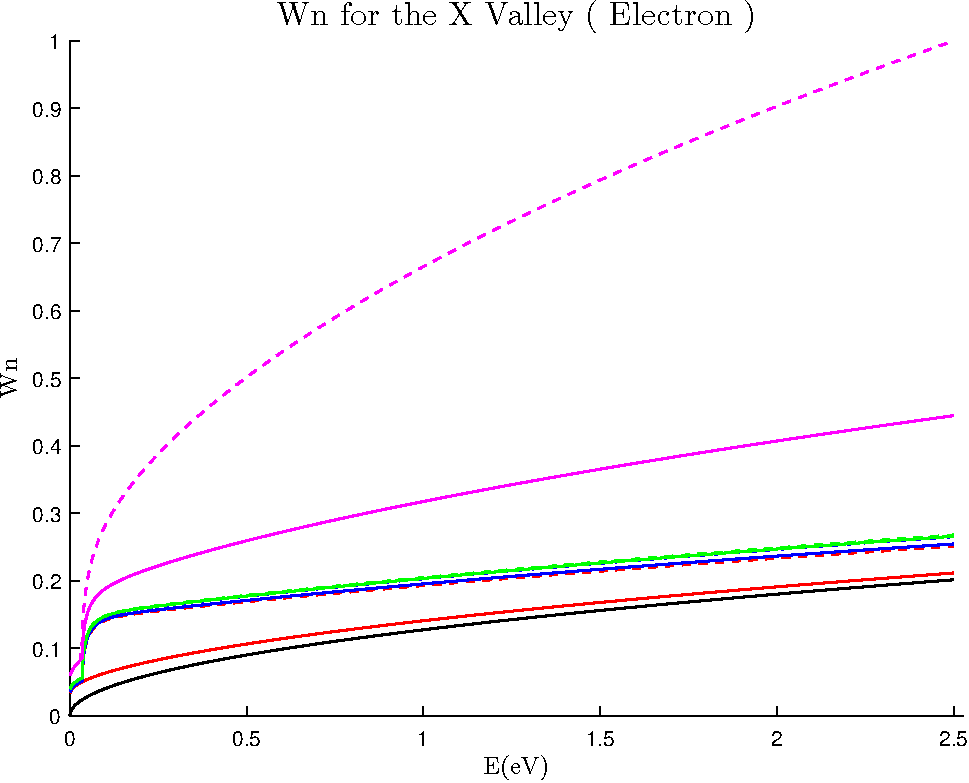
\includegraphics[width=\textwidth]{figures/20250512_130907_Wns_X_valley.pdf}
      \caption{accumulated scattering rates for X valley}
      %\label{fig:graphene-band-surfaces2}
  \end{subfigure}
\end{figure}

\section*{Problem 2}
The time evolution of the $<v_z>$ for different valley as well as the whole ensemble, and the $v_x, v_y, v_z$ at $E_z = 5000 $ V/nm are shown below.
\begin{figure}[htbp]
  \centering
  \begin{subfigure}[b]{0.45\textwidth}
      \centering
      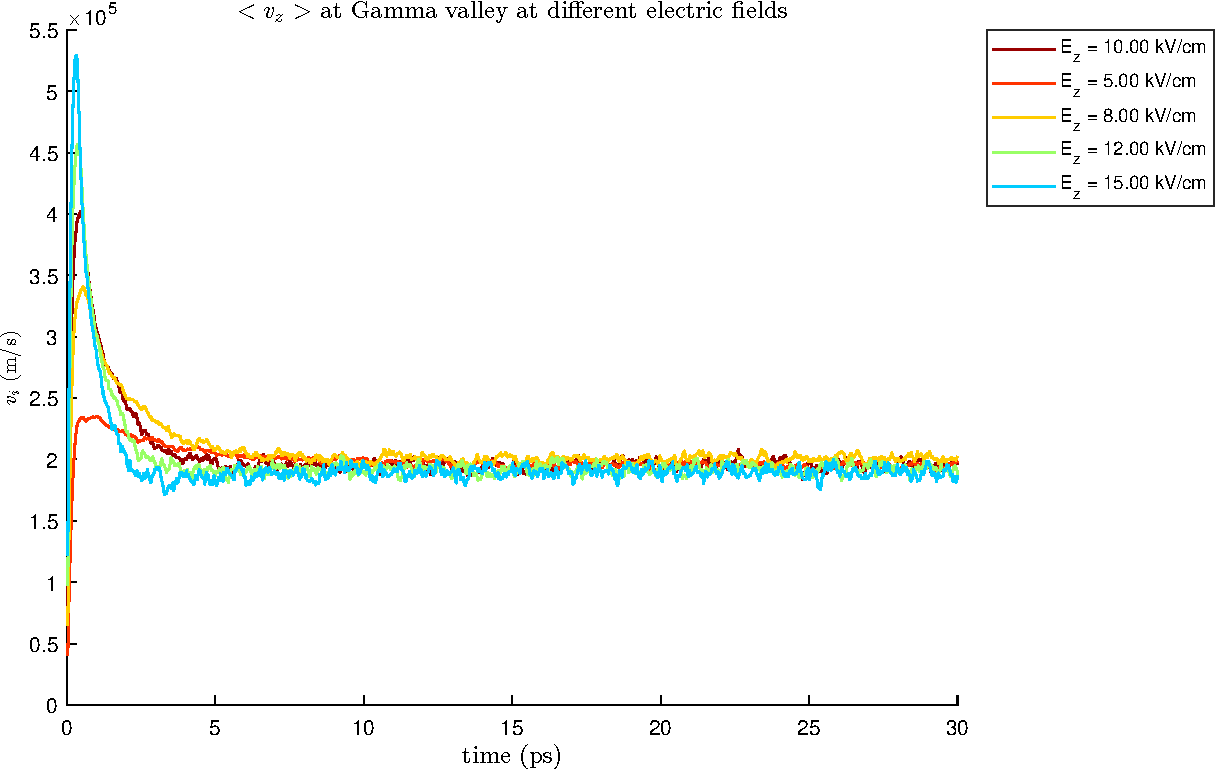
\includegraphics[width=\textwidth]{figures/20250513_211244_vel_time_all_curves_valley01.pdf}
      \caption{$<v_z>$ at G valley}
      %\label{fig:graphene-band-surfaces2}
  \end{subfigure}
  \hfill % 增加水平间距
  \begin{subfigure}[b]{0.45\textwidth}
      \centering
      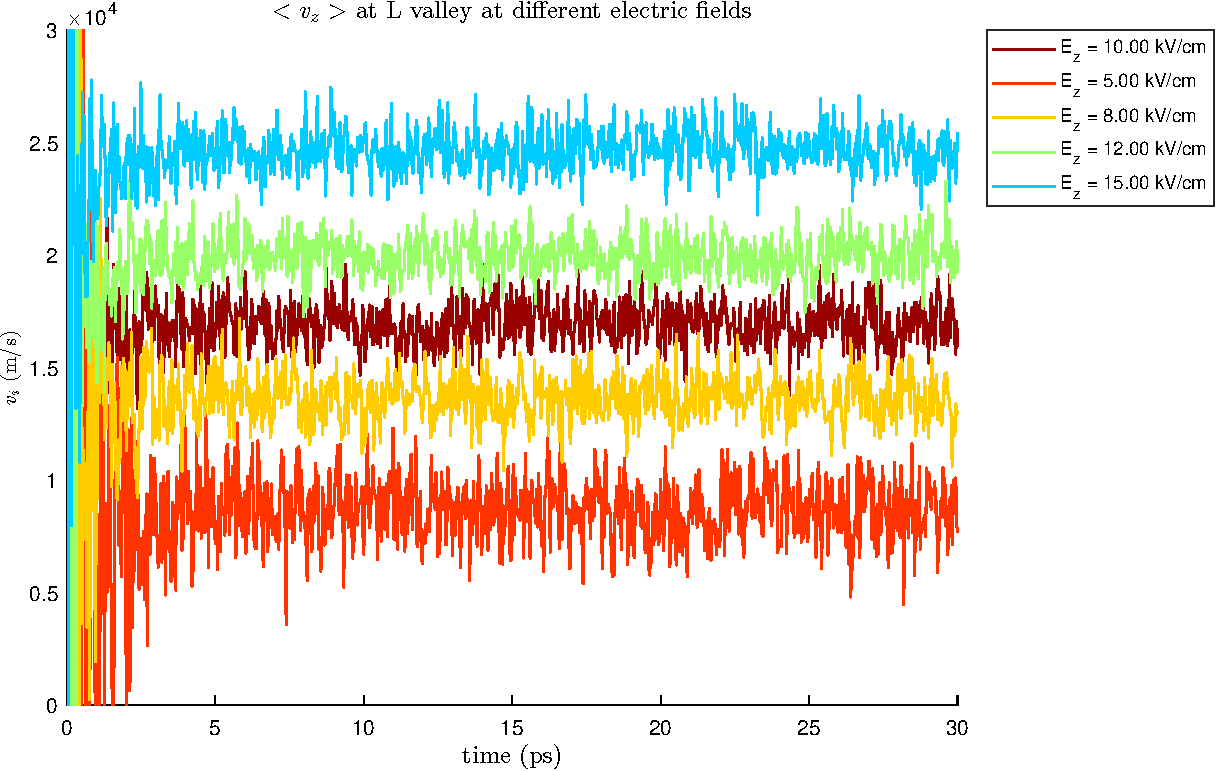
\includegraphics[width=\textwidth]{figures/20250513_211244_vel_time_all_curves_valley02.pdf}
      \caption{$<v_z>$ at L valley}
      %\label{fig:graphene-band-surfaces2}
  \end{subfigure}
  \hfill % 增加水平间距
  \begin{subfigure}[b]{0.45\textwidth}
      \centering
      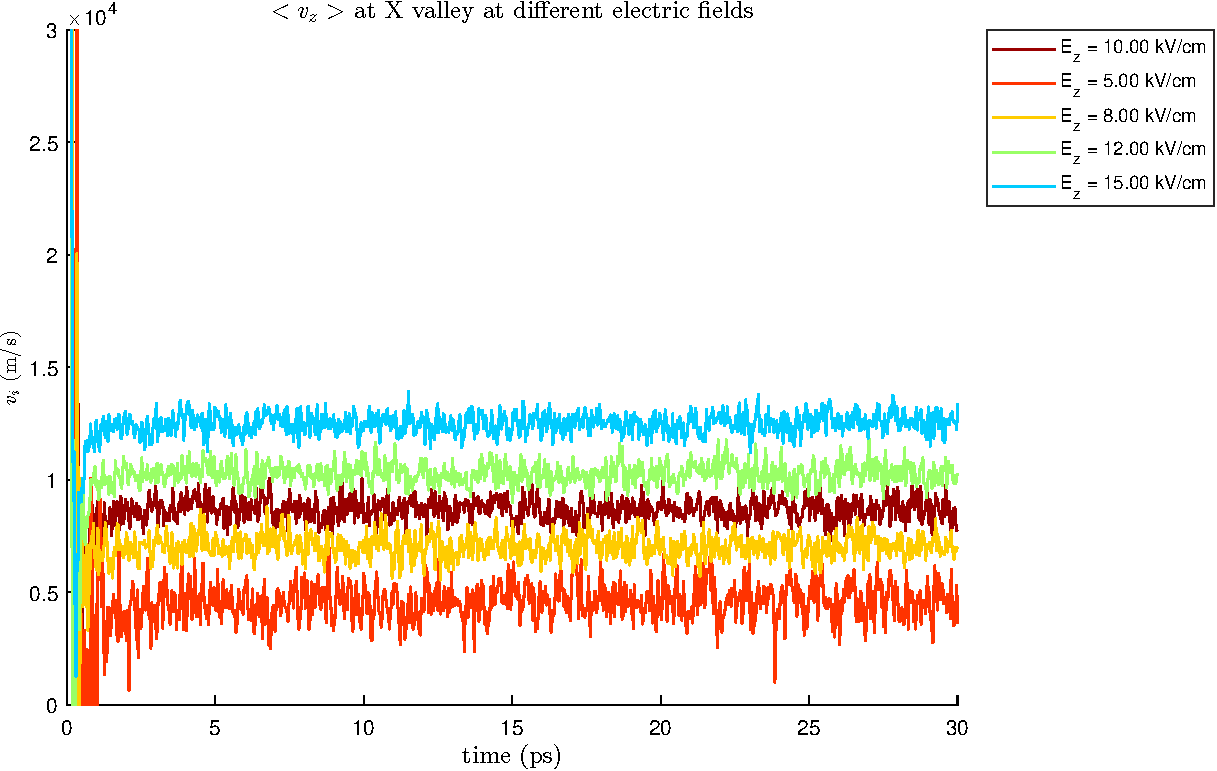
\includegraphics[width=\textwidth]{figures/20250513_211244_vel_time_all_curves_valley03.pdf}
      \caption{$<v_z>$ at X valley}
      %\label{fig:graphene-band-surfaces2}
  \end{subfigure}
  \hfill % 增加水平间距
  \begin{subfigure}[b]{0.45\textwidth}
      \centering
      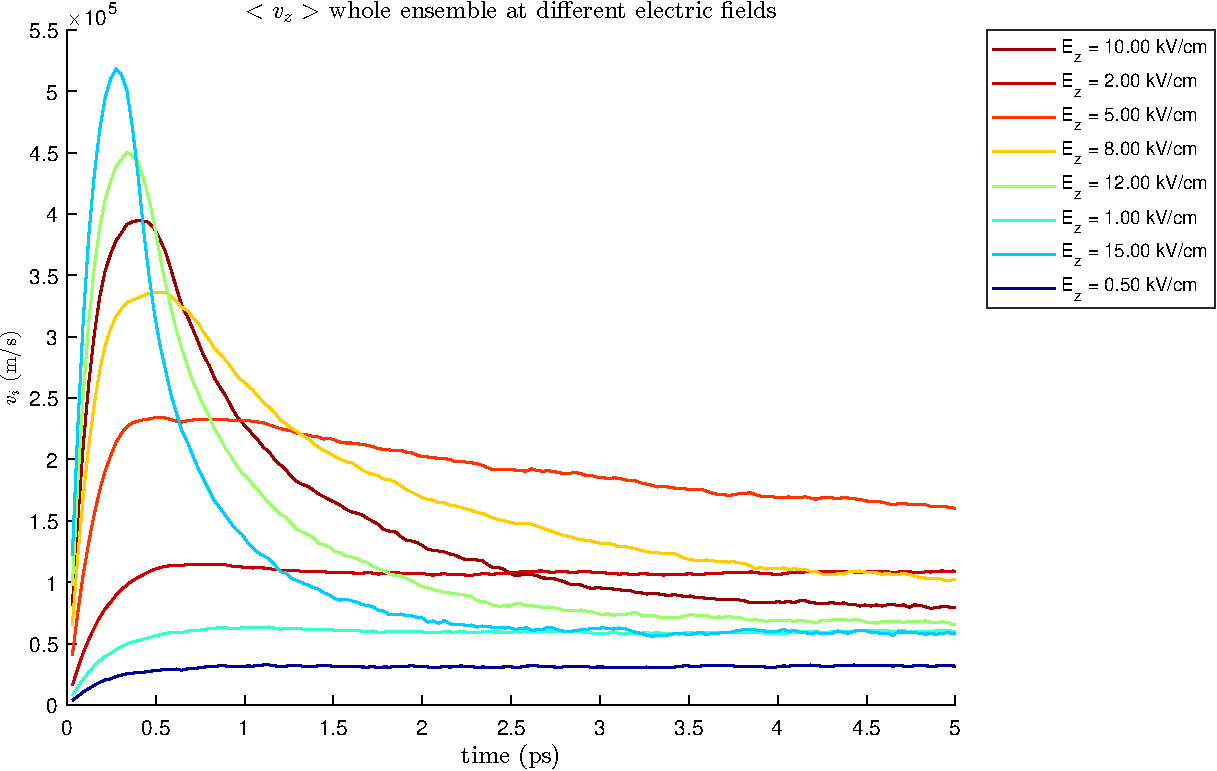
\includegraphics[width=\textwidth]{figures/20250513_224937_vel_time_all_curves_valley04}
      \caption{$<v_z>$ over the whole ensemble}
      %\label{fig:graphene-band-surfaces2}
  \end{subfigure}
  \caption{}
\end{figure}

\begin{figure}[htbp]
  \centering
  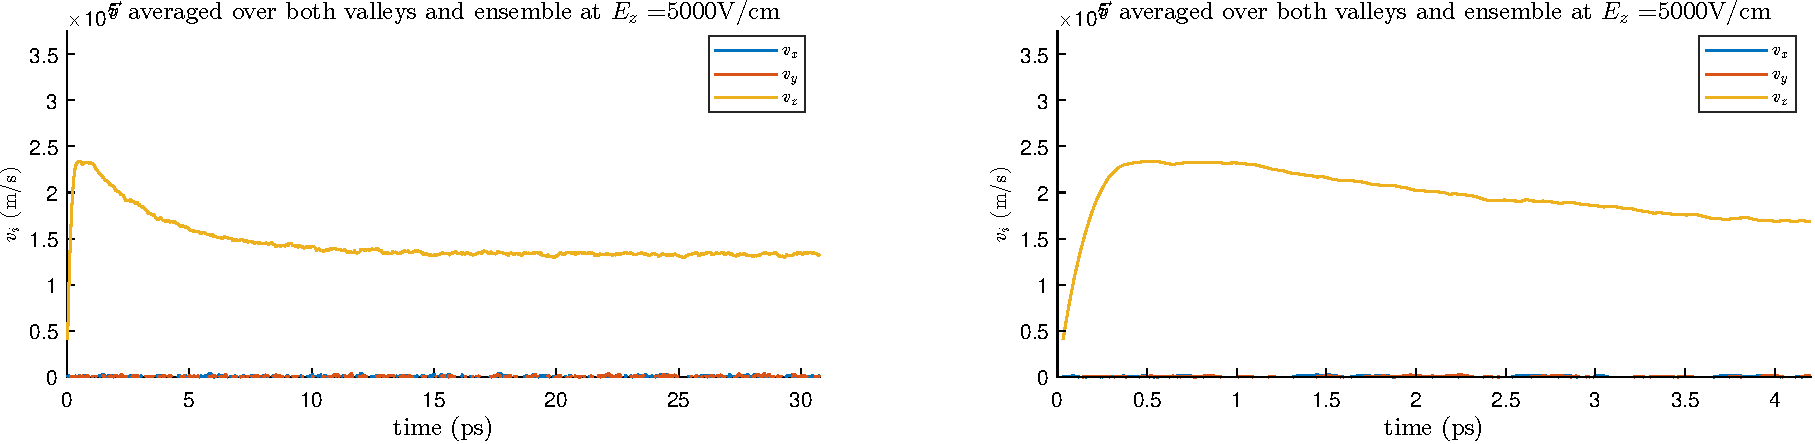
\includegraphics[width=\textwidth]{figures/20250513_200850_Ez_5000V_cm_velocity_avg_all.pdf}
  \caption{$<v_x>, <v_y>, <v_z>$ at $E_z = 5000 $ V/nm}
\end{figure}

Next, let's look at the time evolution of averaged kinetic energy $<E_k>$ for different valley as well as the whole ensemble.
\begin{figure}[htbp]
  \centering
  \begin{subfigure}[b]{0.45\textwidth}
      \centering
      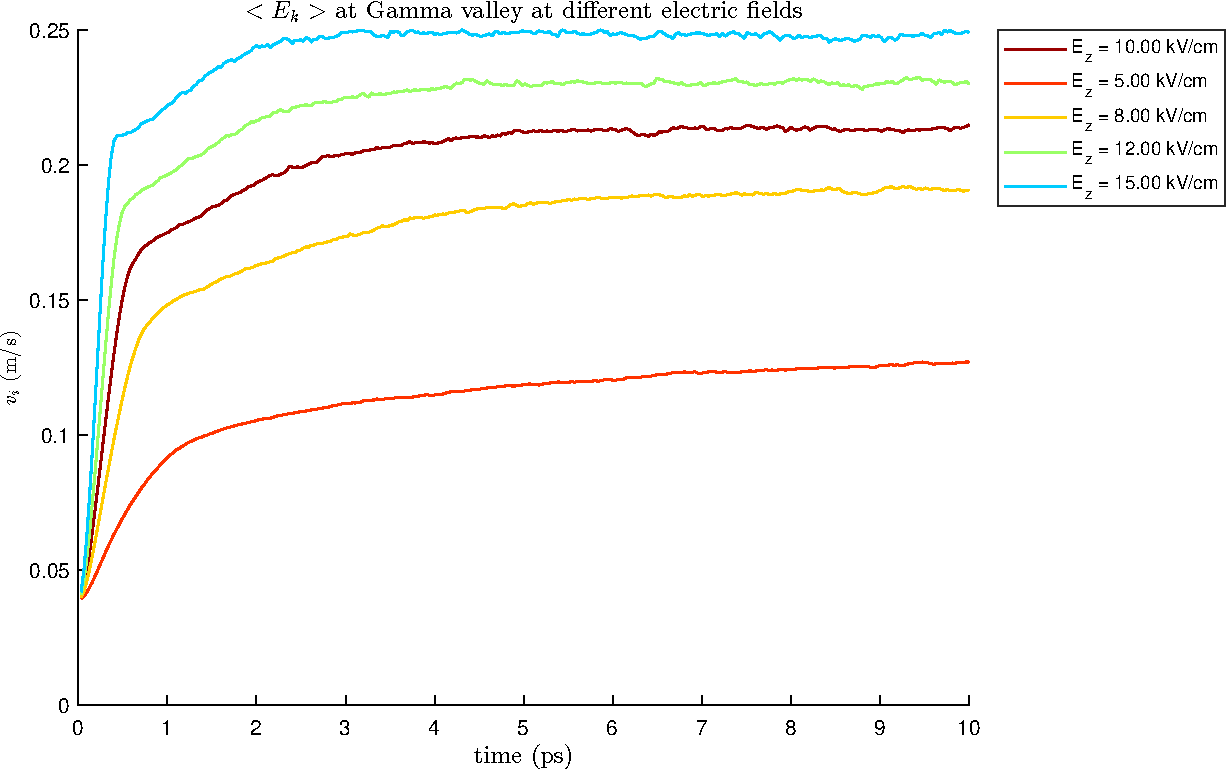
\includegraphics[width=\textwidth]{figures/20250513_211244_ene_time_all_curves_valley01.pdf}
      \caption{$<E_k>$ at G valley}
      %\label{fig:graphene-band-surfaces2}
  \end{subfigure}
  \hfill % 增加水平间距
  \begin{subfigure}[b]{0.45\textwidth}
      \centering
      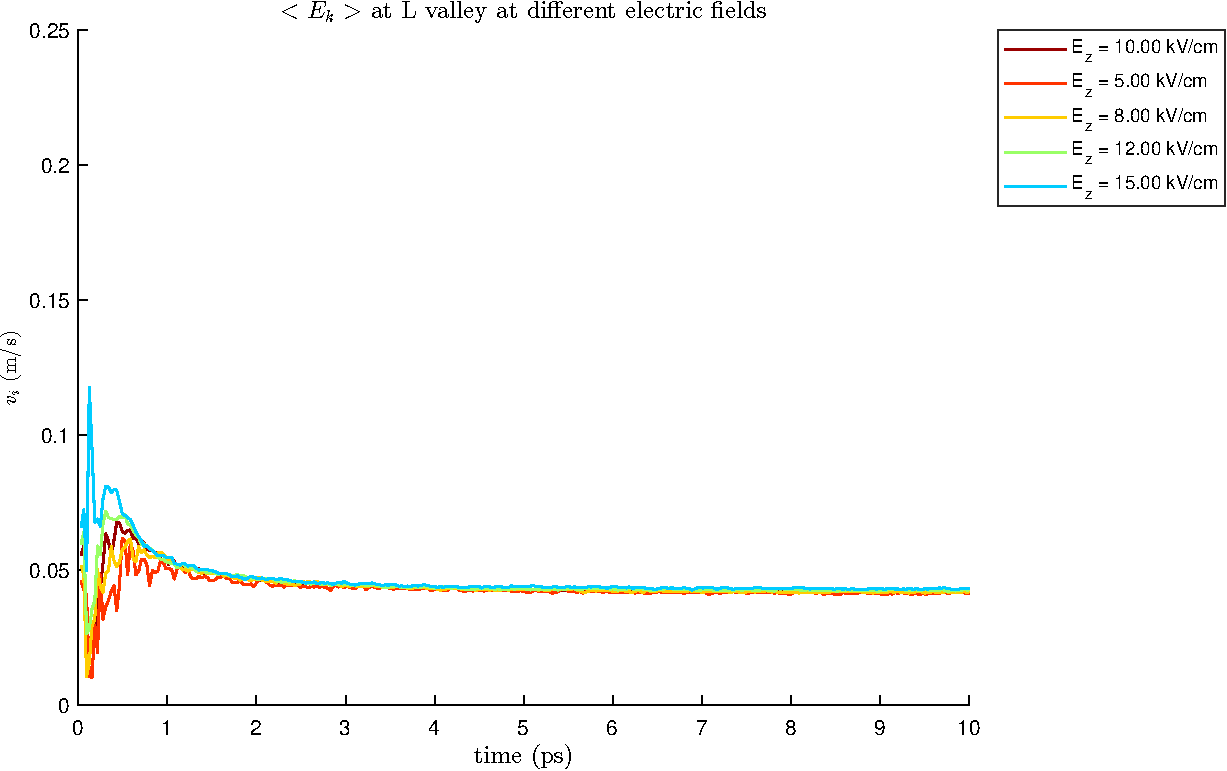
\includegraphics[width=\textwidth]{figures/20250513_211244_ene_time_all_curves_valley02.pdf}
      \caption{$<E_k>$ at L valley}
      %\label{fig:graphene-band-surfaces2}
  \end{subfigure}
  \hfill % 增加水平间距
  \begin{subfigure}[b]{0.45\textwidth}
      \centering
      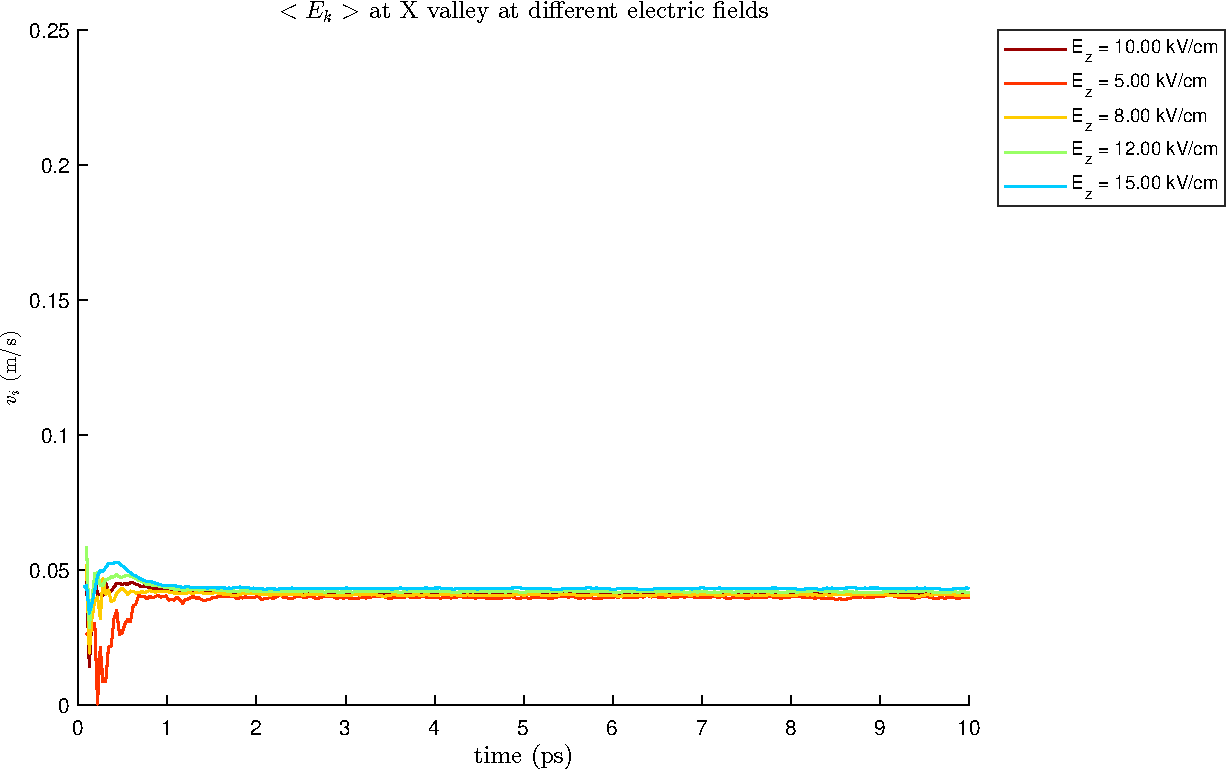
\includegraphics[width=\textwidth]{figures/20250513_211244_ene_time_all_curves_valley03.pdf}
      \caption{$<E_k>$ at X valley}
      %\label{fig:graphene-band-surfaces2}
  \end{subfigure}
  \hfill % 增加水平间距
  \begin{subfigure}[b]{0.45\textwidth}
      \centering
      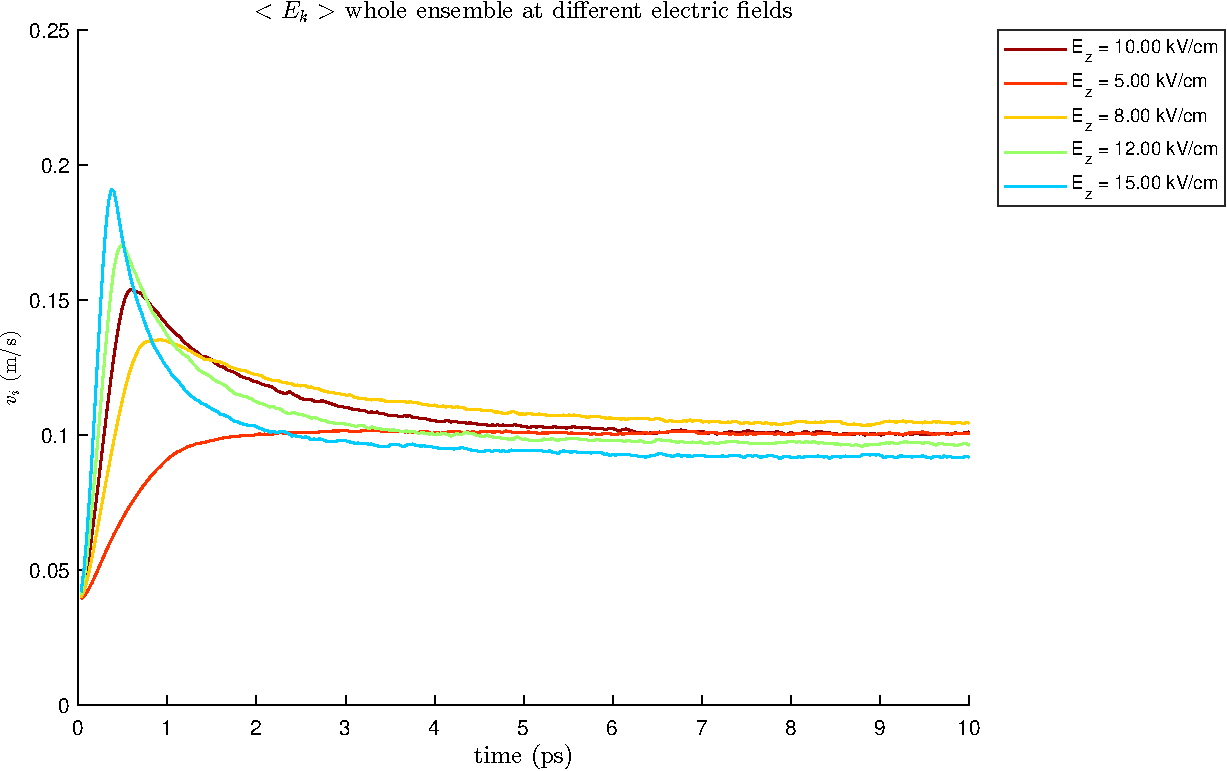
\includegraphics[width=\textwidth]{figures/20250513_211244_ene_time_all_curves_valley04.pdf}
      \caption{$<E_k>$ over the whole ensemble}
      %\label{fig:graphene-band-surfaces2}
  \end{subfigure}
  \caption{}
\end{figure}

Next, let's look at the time evolution of averaged occupation $<N_v>$ for different valley as well as the whole ensemble.
\begin{figure}[htbp]
  \centering
  \begin{subfigure}[b]{0.45\textwidth}
      \centering
      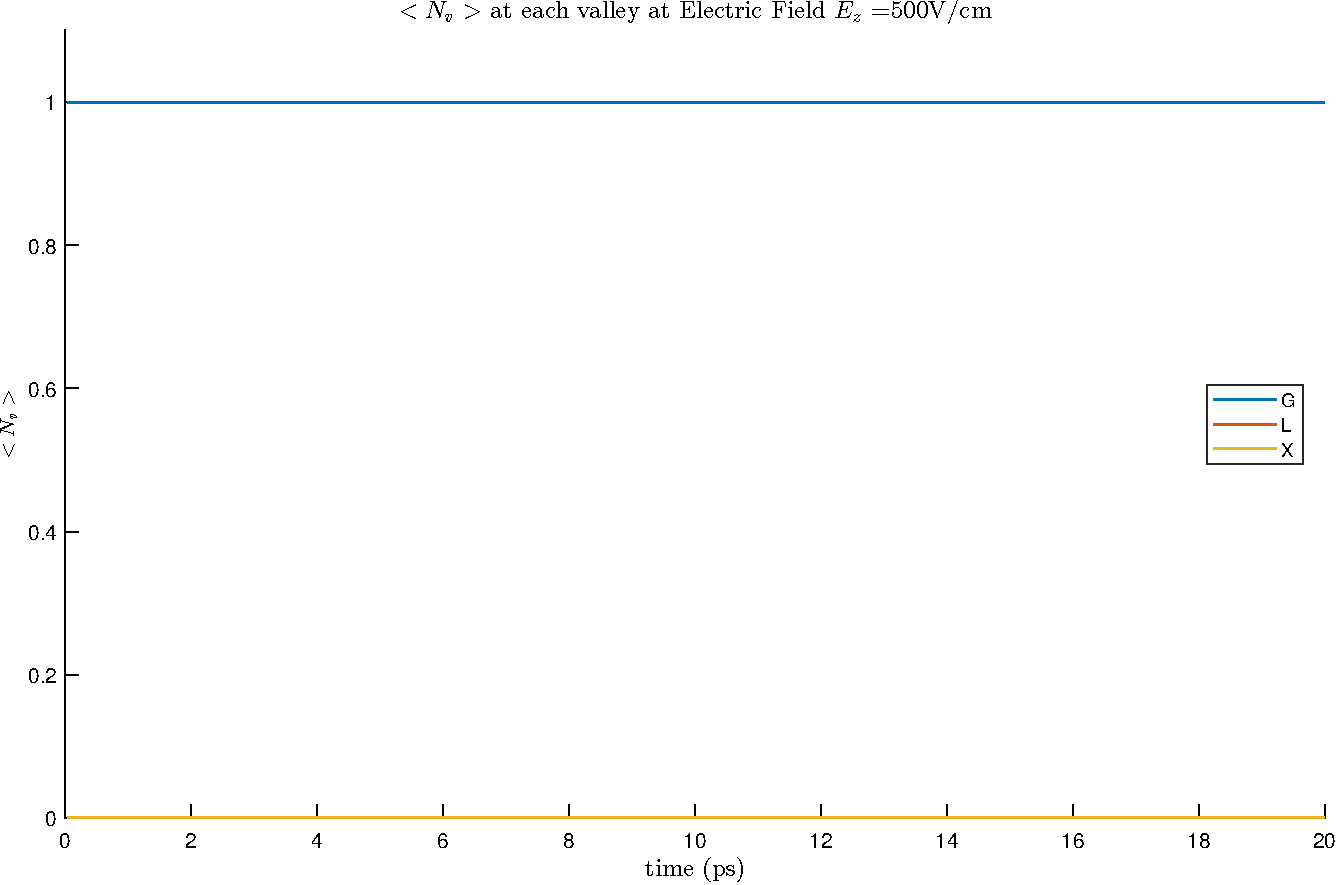
\includegraphics[width=\textwidth]{figures/20250513_211244_Ez_500V_cm_energy_pop.pdf}
      \caption{$<N_v>$ at $500$ V/cm}
      %\label{fig:graphene-band-surfaces2}
  \end{subfigure}
  \hfill % 增加水平间距
  \begin{subfigure}[b]{0.45\textwidth}
      \centering
      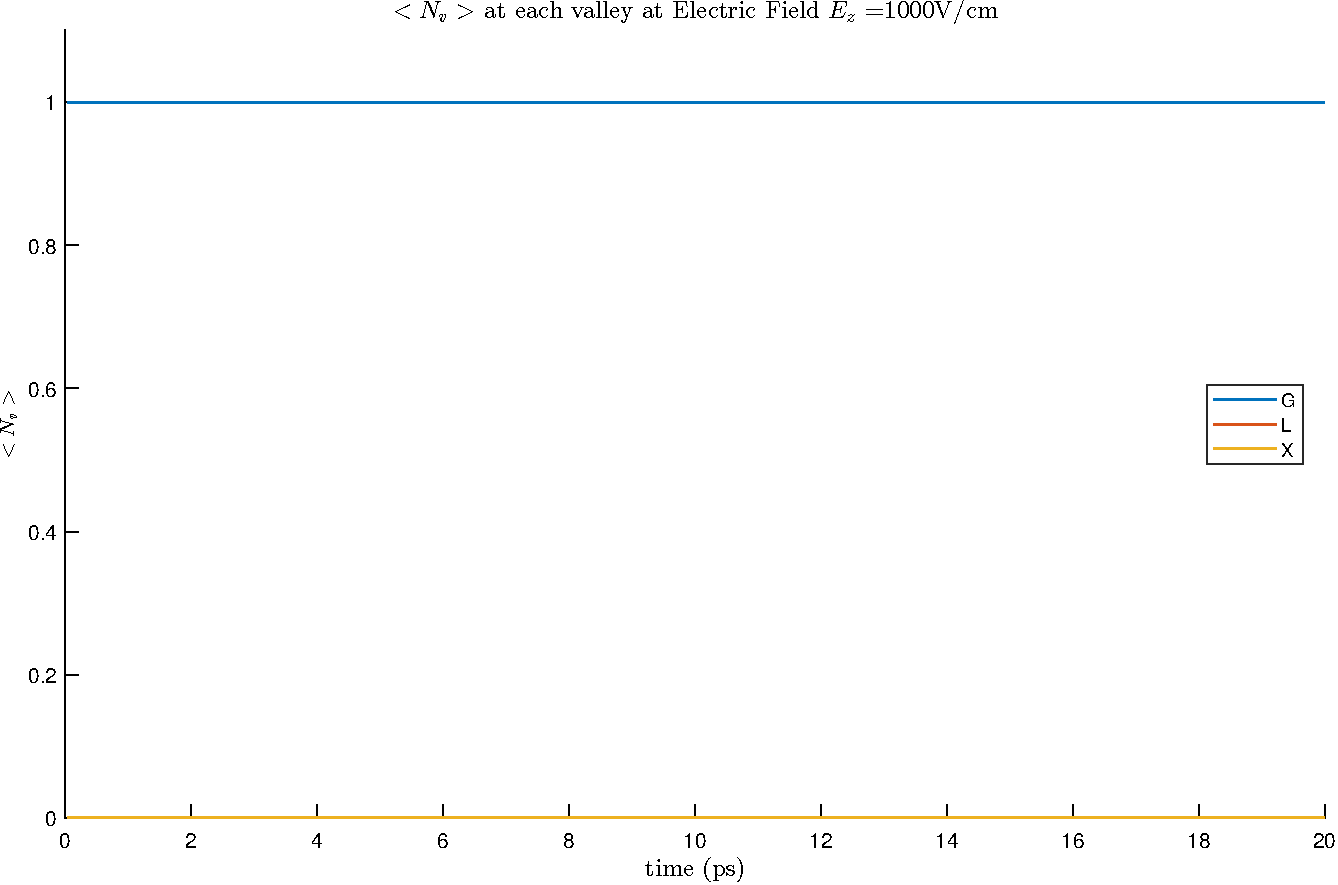
\includegraphics[width=\textwidth]{figures/20250513_211244_Ez_1000V_cm_energy_pop.pdf}
      \caption{$<N_v>$ at $1000$ V/cm}
      %\label{fig:graphene-band-surfaces2}
  \end{subfigure}
  \hfill % 增加水平间距
  \begin{subfigure}[b]{0.45\textwidth}
      \centering
      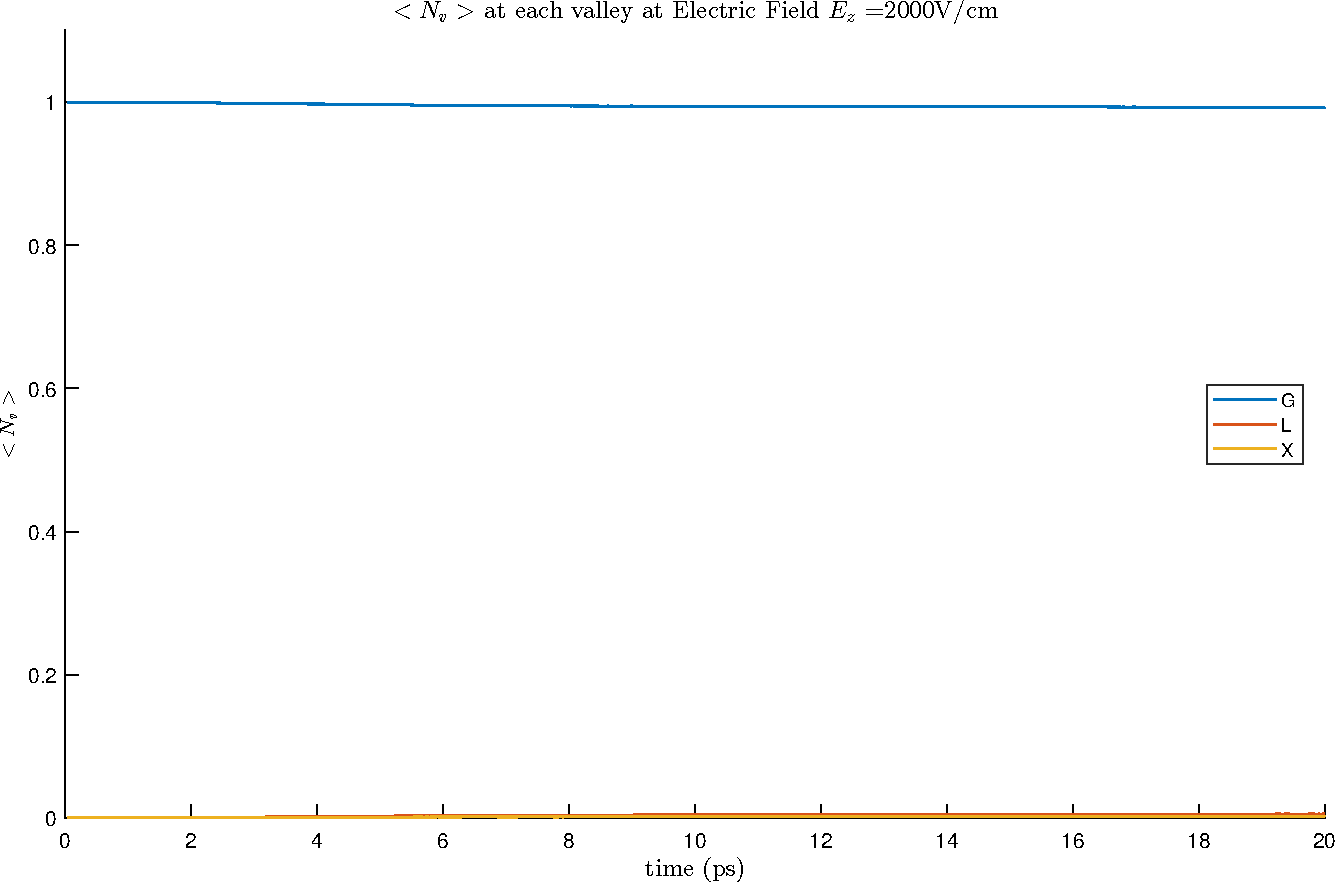
\includegraphics[width=\textwidth]{figures/20250513_200850_Ez_2000V_cm_energy_pop.pdf}
      \caption{$<N_v>$ at $2000$ V/cm}
      %\label{fig:graphene-band-surfaces2}
  \end{subfigure}
  \hfill % 增加水平间距
  \begin{subfigure}[b]{0.45\textwidth}
      \centering
      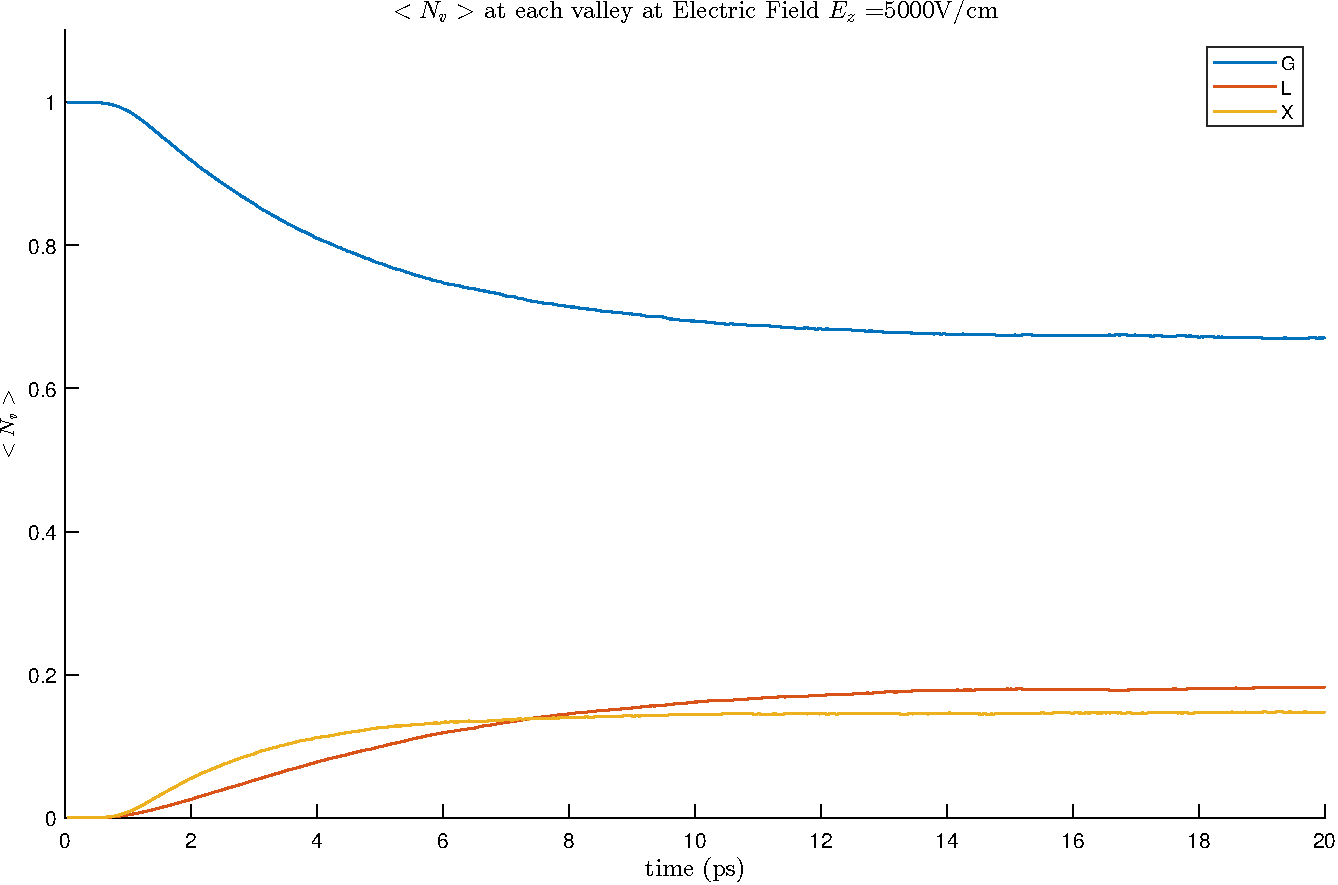
\includegraphics[width=\textwidth]{figures/20250513_200850_Ez_5000V_cm_energy_pop.pdf}
      \caption{$<N_v>$ at $5000$ V/cm}
      %\label{fig:graphene-band-surfaces2}
  \end{subfigure}
  \caption{}
\end{figure}
\newpage

\begin{figure}[htbp]
  \centering
  \begin{subfigure}[b]{0.45\textwidth}
      \centering
      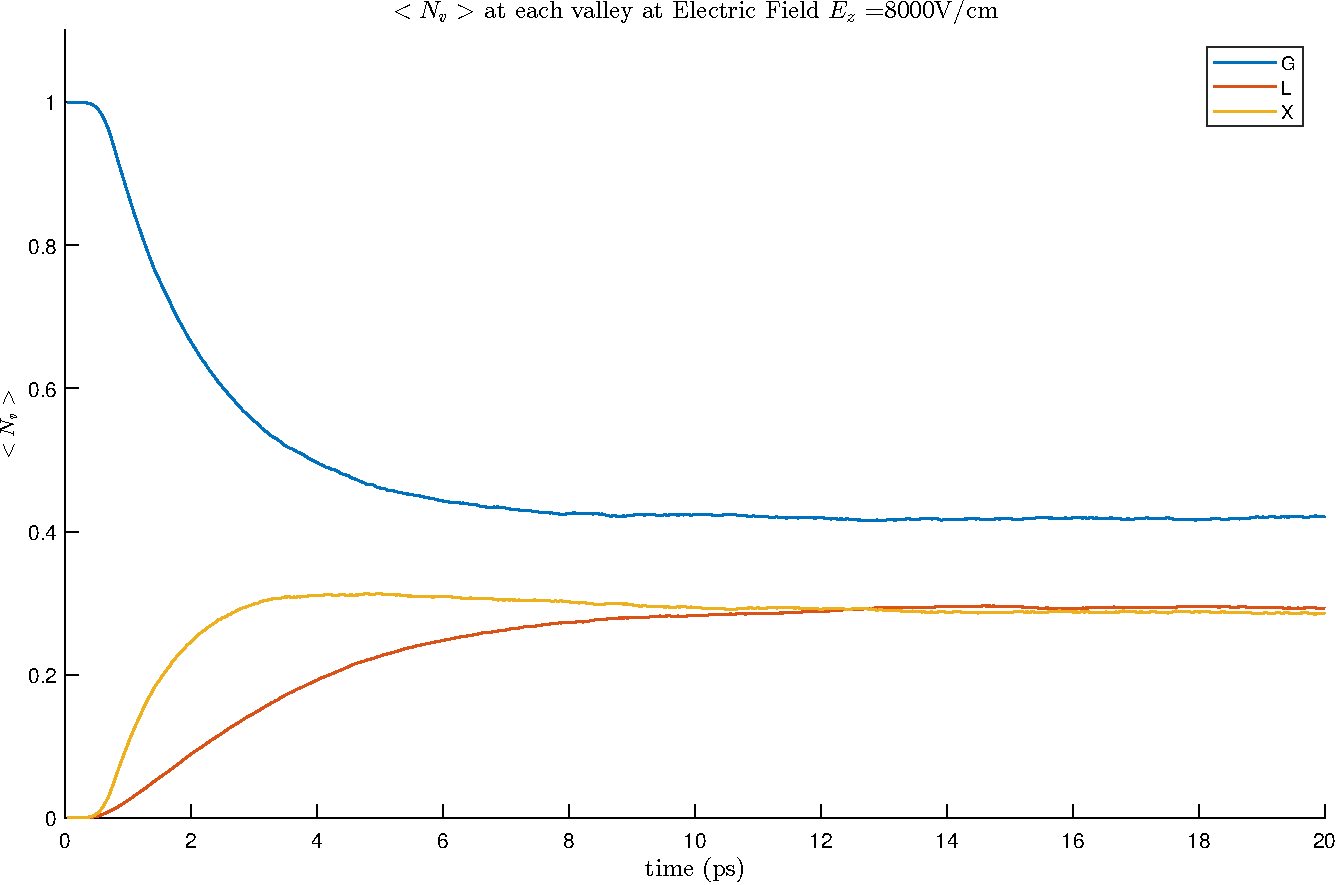
\includegraphics[width=\textwidth]{figures/20250513_200850_Ez_8000V_cm_energy_pop.pdf}
      \caption{$<N_v>$ at $8000$ V/cm}
      %\label{fig:graphene-band-surfaces2}
  \end{subfigure}
  \hfill % 增加水平间距
  \begin{subfigure}[b]{0.45\textwidth}
      \centering
      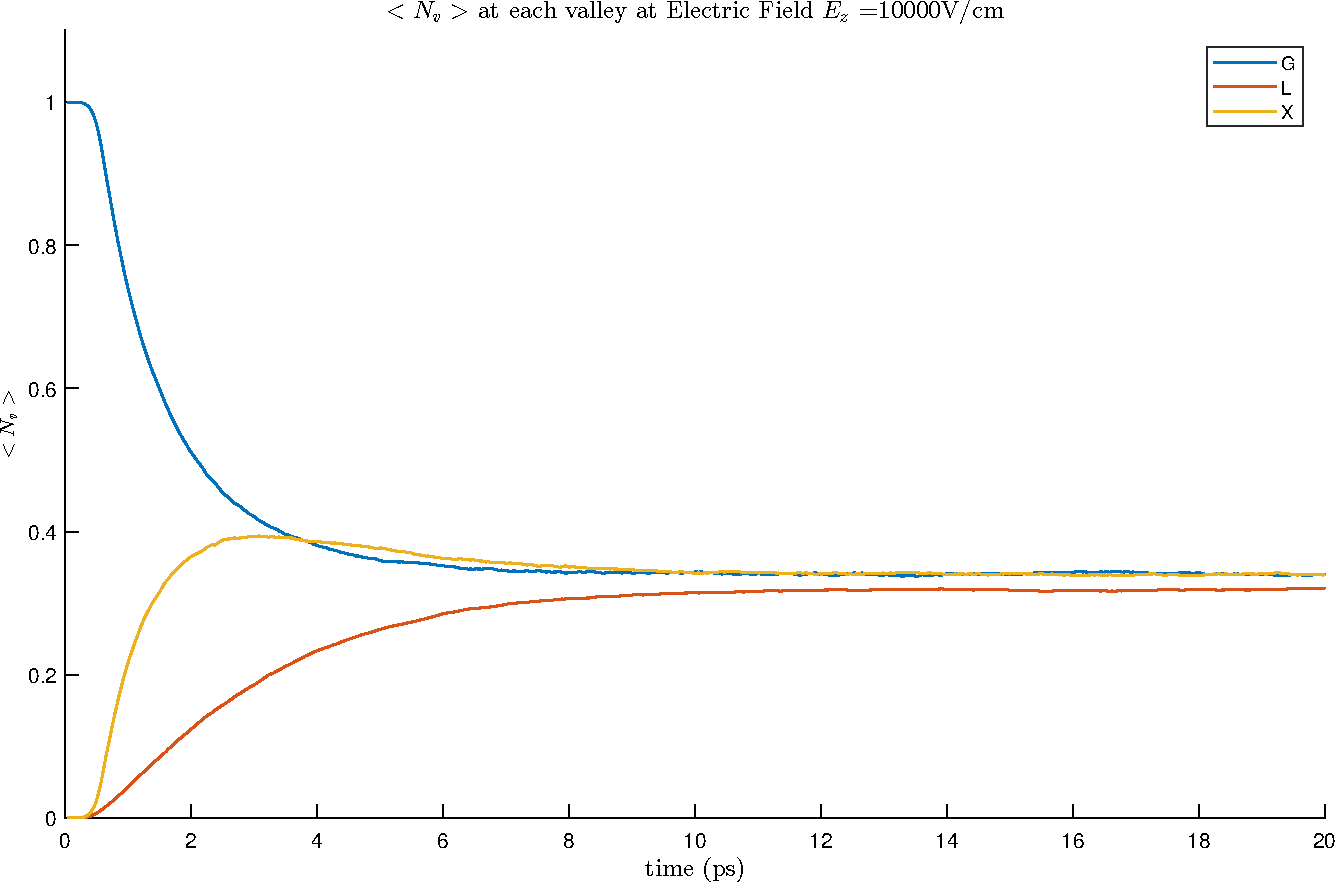
\includegraphics[width=\textwidth]{figures/20250513_200850_Ez_10000V_cm_energy_pop.pdf}
      \caption{$<N_v>$ at $10000$ V/cm}
      %\label{fig:graphene-band-surfaces2}
  \end{subfigure}
  \hfill % 增加水平间距
  \begin{subfigure}[b]{0.45\textwidth}
      \centering
      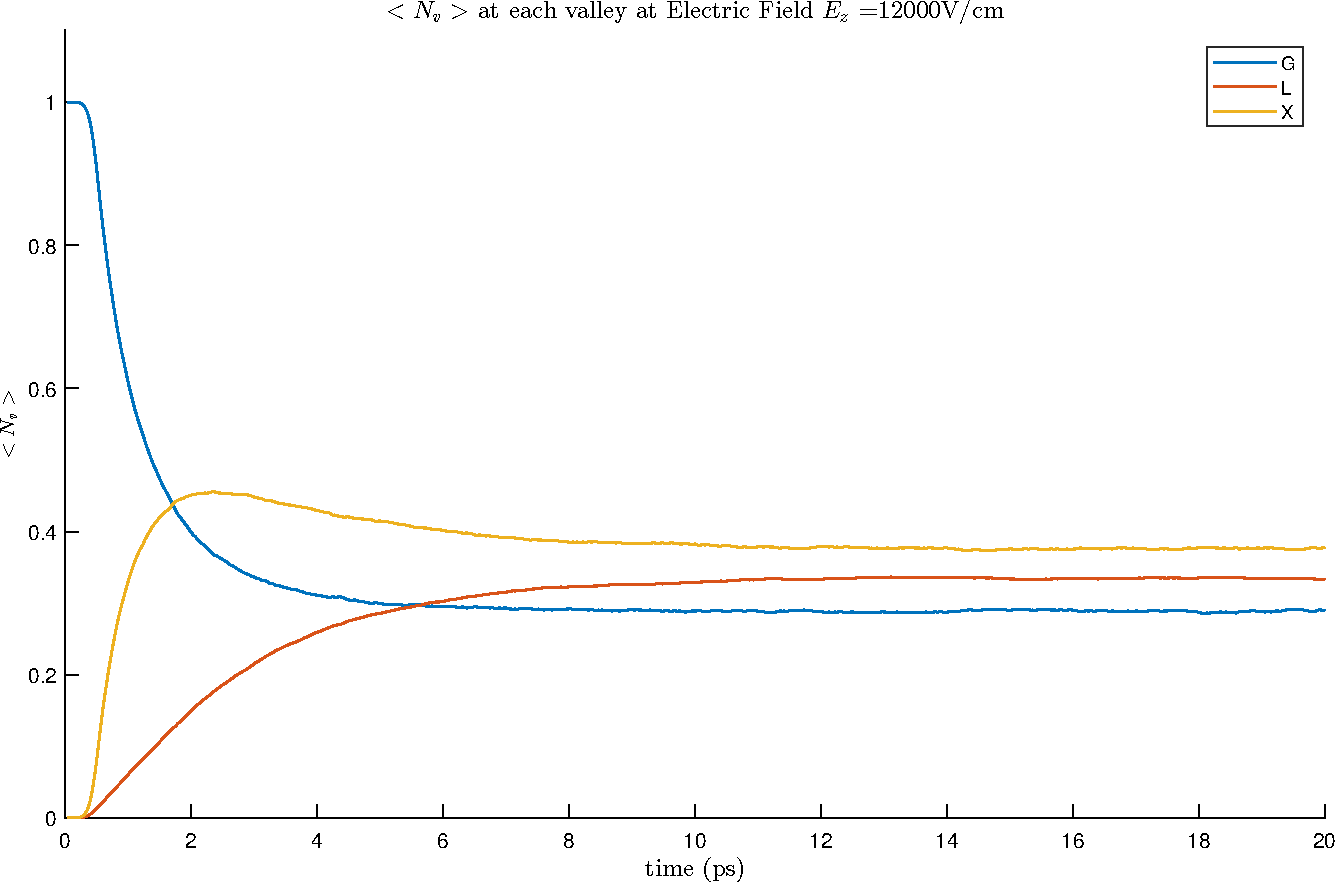
\includegraphics[width=\textwidth]{figures/20250513_205236_Ez_12000V_cm_energy_pop.pdf}
      \caption{$<N_v>$ at $12000$ V/cm}
      %\label{fig:graphene-band-surfaces2}
  \end{subfigure}
  \hfill % 增加水平间距
  \begin{subfigure}[b]{0.45\textwidth}
      \centering
      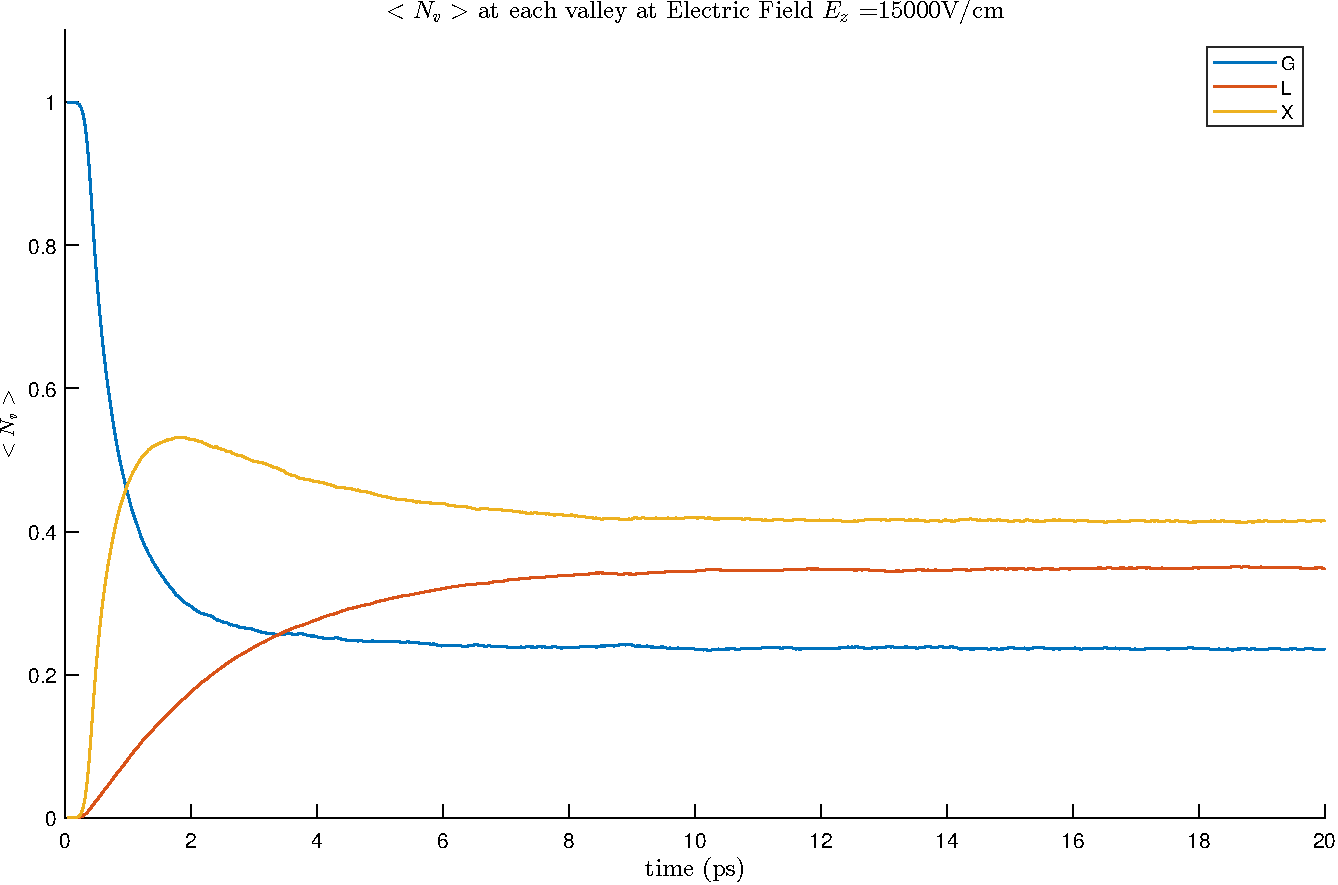
\includegraphics[width=\textwidth]{figures/20250513_211244_Ez_15000V_cm_energy_pop}
      \caption{$<N_v>$ at $15000$ V/cm}
      %\label{fig:graphene-band-surfaces2}
  \end{subfigure}
  \caption{}
\end{figure}

\newpage
\section*{Problem 3}
The steady state velocity, energy, and occupations as a function of electric field are shown below.
\begin{figure}[htbp]
  \centering
  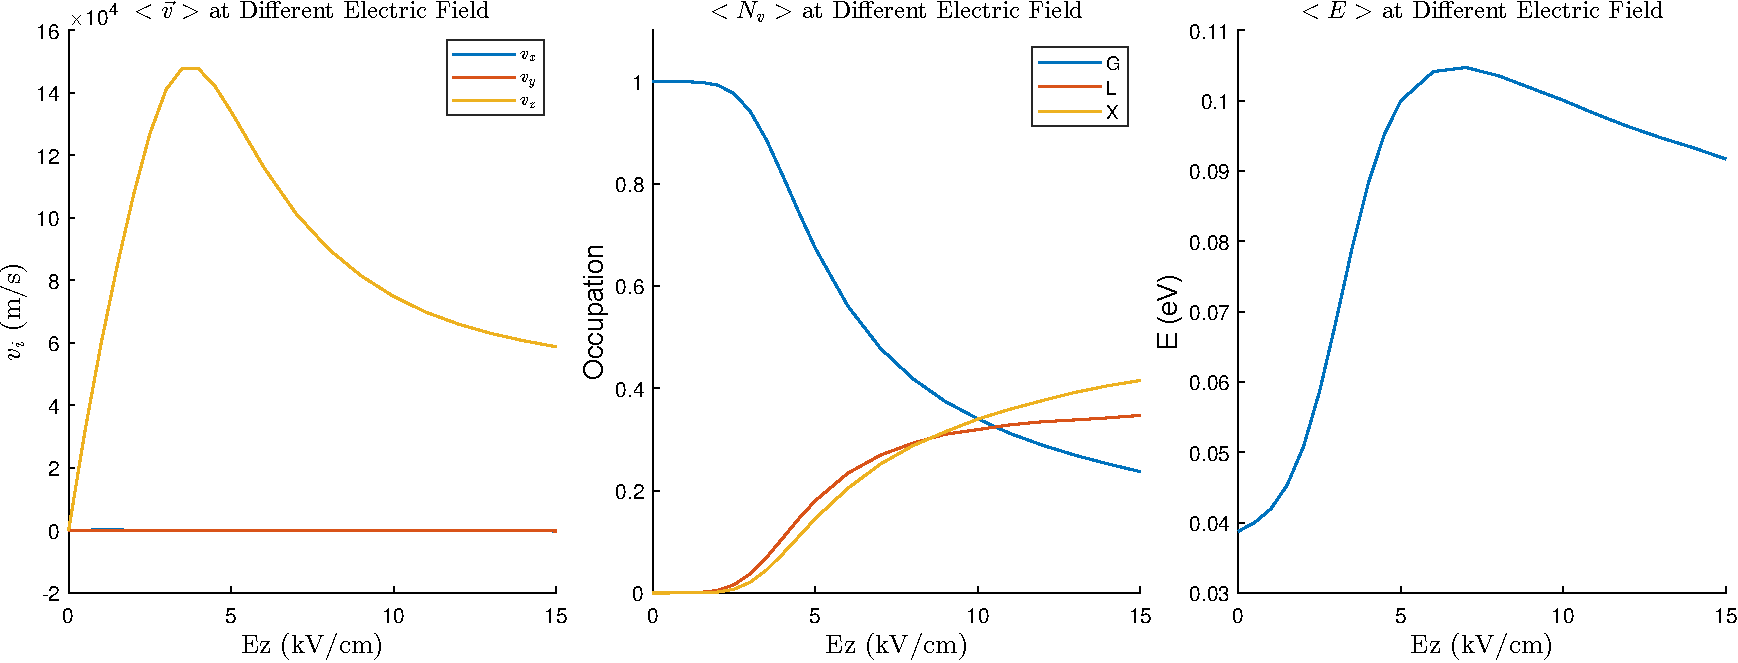
\includegraphics[width=\textwidth]{figures/20250513_211244_vel_pop_ene_Ez.pdf}
  \caption{steady behavior as a function of electric field}
\end{figure}
By linear fitting, the low-field mobility is $3300$ cm$^2$/V$\cdot$s, which is smaller than the values in textbook. Maybe because of the neglect of other scattering mechanisms and anharmonic electronic structure.

\end{document}